% !TeX root = ../main.tex
% Add the above to each chapter to make compiling the PDF easier in some editors.

\chapter{Training}\label{chapter:Training}
This chapter first describes the default setup of the network and the training task. Followed by the specification of the target and its trajectory. Afterwards the specifics of the different experiment setups are described as well as the results of the training phase.
\section{Structure and Parameters of the Network}
In this thesis SNNs in different topologies as well as with different parameter settings are going to be tested. First the simplest topology is used consisting of ten poisson neurons, ten LIF input neurons and two LIF output neurons with each a spike detector connected. \autoref{fig:simpleNetwork} shows a schematic of the network where all but the connections between the input and hidden are static and only between the LIF neurons R-STDP synapses are used. The input layer of LIF neurons are set up to parrot the spikes from the poisson neurons and is necessary as the poisson layer is defined by the transfer functions and thus connections to it can not be described in the simulation setup of the network. To produce this behaviour of the neurons their refractory period is set to zero and their threshold voltage is set close to the resting voltage. The exact parameters are shown in \autoref{tab:parrotPar}.


\begin{figure}[htpb]
  \centering
  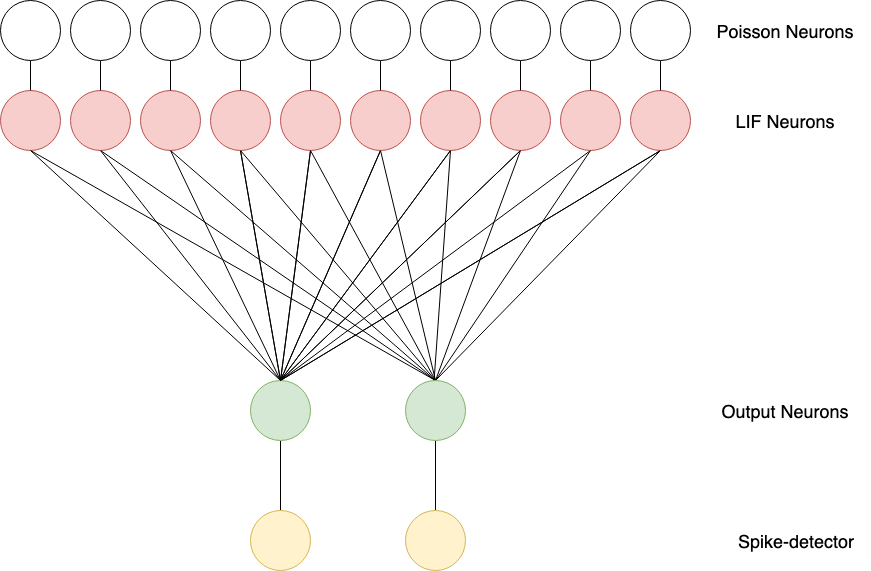
\includegraphics[width=\textwidth]{figures/plots/simpleNetwork}
  \caption [Simple Network]{This figure shows the Simplest Network Topology used for simulations}
  \label{fig:simpleNetwork}
\end{figure}

\begin{table}[htpb]
\caption[Parameters Parrot Neuron]{Parameters of Parrot Neurons} \label{tab:parrotPar}
\centering
\begin{tabular}{|c| c |l|}
    \toprule
    Parameter & Value & Description \\
    \midrule
    $c_m$   & 1.0  & Capacity of the membrane \\
    $tau_{m}$    & 20.0  & Membrane time constant \\
    $tau_{refrac}$   & 0.  & Duration of refractory period\\
    $v_{thresh}$   & -64.50  & Spike initiation threshold \\
    $v_{reset}$    & -65.0  &  Reset value for $V_m$ after a spike \\
		$v_{rest}$ & -65.0 & Resting voltage \\
    \bottomrule
\end{tabular}
\end{table}

In the output layer the parameters are set to get a behaviour where some spikes are needed to fire the neuron but it still doesn’t fire to sparse. This behaviour is wanted as it somehow defines basic requirements for learning. Are the spikes to rare the synapses connecting to it won’t learn, on the other hand if the neuron fires with every incoming spike the ability to learn is at least strongly hindered as it makes the eligibility mechanism useless. To reduce the impact of a single spike on the potential of the neuron, its capacity can be increased while the time window in which these spikes can appear can be spread by increasing the membrane time constant. The parameters used for the output layer can be seen in \autoref{tab:outputParam}.


\begin{table}[htpb]
  \caption[Parameters Output Neuron]{Parameters of Output Neurons} \label{tab:outputParam}
  \centering
  \begin{tabular}{|c| c |l|}
      \toprule
      Parameter & Value & Description \\
      \midrule
      $c_m$   & 10.0  & Capacity of the membrane \\
      $tau_{m}$    & 50.0  & Membrane time constant \\
      $tau_{refrac}$   & 1.  & Duration of refractory period\\
      $v_{thresh}$   & -50.0  & Spike initiation threshold \\
      $v_{reset}$    & -65.0  &  Reset value for $V_m$ after a spike \\
      $v_{rest}$ & -65.0 & Resting voltage for $V_m$ \\
      \bottomrule
  \end{tabular}
  \end{table}

The parameters for the R-STDP synapses are shown in \autoref{tab:baseRstdp} and are chosen to have only a short memory to the past and a balanced eligibility for the STDP learning windows. The memory timespan is proportional to he eligibility time constant $\tau_c$ which is set to $40$ milliseconds, two times the simulation timestep. The height of the STDP function for a pre-post-spiking pattern is given by $A_+$ and for a post-pre pattern by $A_-$ which are the constant scaling strengths of potentiation and depression and are set to the same value to have an equal impact on the eligibility trace. To achieve stable learning the change in weights shouldn’t be too extreme as the network is unlikely to stabilise in such a scenario. As \autoref{eq:dWrStdp} shows the weight change is proportional to the magnitude of the eligibility trace $c$ and the neuromodulator concentration $n$. Thus the magnitude of the scaling factors $A_{+/-}$, influencing the magnitude of $c$,  have to be balanced with the scaling factor $c_{rew}$ of the reward function shown in \autoref{eq:reward}, influencing the magnitude of $n$. In this experiments the baseline concentration $b$ in \autoref{eq:dWrStdp} is set to zero as the concentration is directly assigned and not regulated through a dopamine neuron. Thus negative values can be assigned which otherwise would result by a lower neuromodulator concentration $n$ than the baseline concentration $b$.

\begin{table}[htpb]
  \caption[Parameters R-STDP synapse]{Parameters of R-STDP Synapse} \label{tab:baseRstdp}
  \centering
  \begin{tabular}{|c| c |l|}
      \toprule
      Parameter & Value & Description \\
      \midrule
      $W_{max}$ & 6000   & Maximum weight of synapse\\   
      $W_{min}$ & -6000  & Minimum weight of synapse\\   
      $A_{+}$   & 0.1    & Constant scaling strength of potentiation\\   
      $A_{-}$   & -0.1   & Constant scaling strength of depression \\   
      $\tau_c$  & 40.0   & Time constant of eligibility trace \\  
      $\tau_n$  & 20.0   & Time constant of reward signal  \\   
      $b$       & 0.0    & Baseline neuromodulator concentration \\    
      \bottomrule
  \end{tabular}
  \end{table}

The angle used for the reward function, which can be seen as the target angle to minimize, is the angle of the head to the ball at each timestep. Further if this angle overcomes $35$ degrees the target and robot get reset to the starting positions and the path of the target gets inverted.
The reward factor $c_{rew}$ in the \autoref{eq:reward} is set to $0.00005$ and the reward is halved every $3000$ time steps which helps the network to better stabilise over time. Stabilisation means that the weights in the network only change to small degree or at best not at all. For this to happen the reward to the network has to be zero or near to it. For the angle from the snakes head to the ball this is not possible for each timestep as result of the movement of the snake. By reducing the reward over time we negate this effect to some degree. The factor $c_{imp}$ in \autoref{eg:OutputCalc} is set to $0.05$, this is scaling the impact of the networks output on the direction. 

\section{Simulation Environment}
For the simulation the robot is placed in an empty environment with a sphere as target which is spawned $1.6$ meters in front of the robot with a radius of $30$ centimeters. The sphere or ball is then moved along a path in an eight shaped form. A schematic of the movement pattern of the ball is shown in \autoref{fig:ballMove}, the directions from one point to the other can be found in \autoref{tab:ballMove} in the appendix.
The target is set to move faster than the snake but won’t move further away from the snake then the initial $1.6$ meters.


\section{Benchmark Experiment}
The previously described setting is used as benchmark or baseline setting for testing the capabilities of the setup. 
The training simulation shows that the network is able to completely solve the task on the third try after $151093$ training steps, $3021.86$ seconds, but still heavily depends on the reward signal. The reliance on reward is visible in the strongly changing weights shown in \autoref{fig:midWBase1}. After completing the second run in inverse direction the training was stopped as the weights seemed to have stabilised as can be seen in \autoref{fig:endWBase1}.

\begin{figure}[htpb]
  \centering
  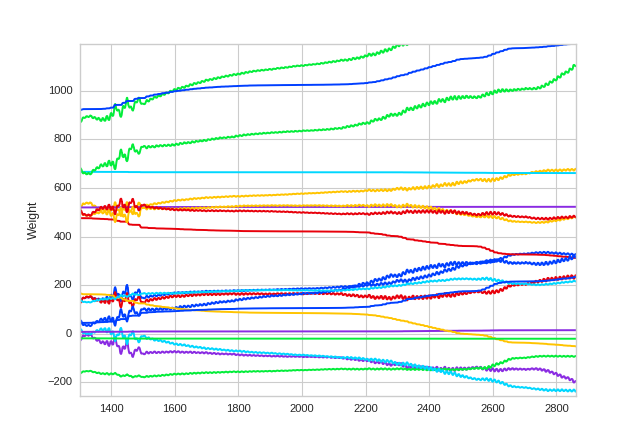
\includegraphics[width=\textwidth]{figures/plots/newPlots/base1Training_weights_mid}%midWBase1}
  \caption{Change of weights while still learning }
  \label{fig:midWBase1}
\end{figure}


\begin{figure}[htpb]
  \centering
  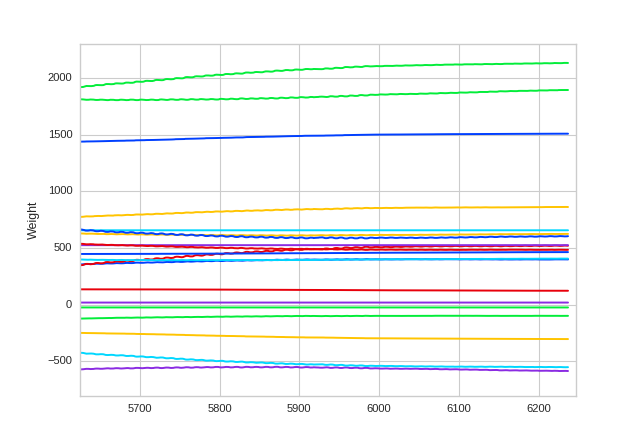
\includegraphics[width=\textwidth]{figures/plots/newPlots/base1Training_weights_end}%endWBase1}
  \caption{Change of weights at end of learning period }
  \label{fig:endWBase1}
\end{figure}
\autoref{fig:WBase1} shows the graph of the weights over the whole training period where \autoref{fig:dopeBase1} and \autoref{fig:angleBase1} show the graphs for reward given to the network and the mean angle and distance to the target over time.

\begin{figure}[htpb]
  \centering
  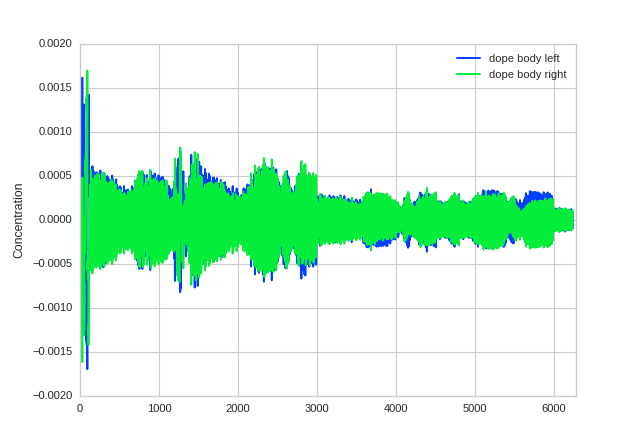
\includegraphics[width=\textwidth]{figures/plots/newPlots/base1Training_reward}%dopeBase1}
  \caption{ Complete plot of the reward }
  \label{fig:dopeBase1}
\end{figure}
\begin{figure}[htpb]
  \centering
  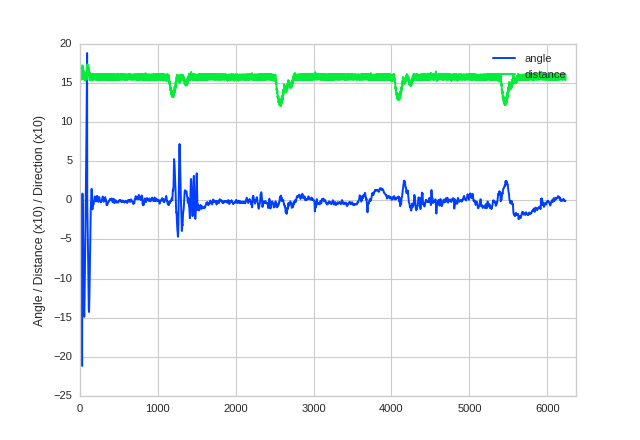
\includegraphics[width=\textwidth]{figures/plots/newPlots/base1Training_perf}%angleBase1}
  \caption{ Complete plot of the mean angle and distance to the Target }
  \label{fig:angleBase1}
\end{figure}
\begin{figure}[htpb]
  \centering
  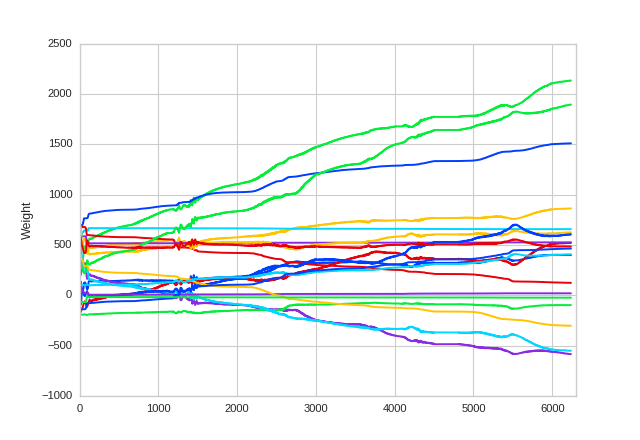
\includegraphics[width=\textwidth]{figures/plots/newPlots/base1Training_weights}%WBase1}
  \caption{ Complete plot of the weights for the base simulation }
  \label{fig:WBase1}
\end{figure}

\section{Single Layer Network with Head Control}
As follow up task, the network should control the robot direction and additionally the direction the head of the snake is facing. To control the head an additional pair of output neurons is added steering the head in a similar fashion to the other two neurons, described in \autoref{sec:OutputDecoding}. For this setup the factors scaling the impact of the output on the directions in the \autoref{eg:OutputCalc} are set to 0.02 for the head and $0.07$ for the body.
The reward assigned to the neurons controlling the head is as before corresponding to the angle of the head to the target, $a_{head}$, at each timestep. For the body the reward is proportional to the angle of the body to the target $a_{body}$ which is calculated by
\begin{equation} \label{eq:bodyAngle}
a_{body} = a_{head} - d_{head}
\end{equation}
where $d_{head}$ is the direction of the head at that point. This is the angle the snake head would have if it would always face forward.
In this simulation the robot gets reset if the absolute value of either $a_{head}$ is bigger than $40$ degrees or the mean angle of the body is greater than $35$ degrees.
The mean value of the angle is calculated over the past $625$ simulation steps which corresponds to $12.5$ seconds which is the length of one movement period of the snake, meaning in $12.5$ seconds the head will move from one end to the other and back. 
\begin{equation}
A_{mean} = \frac { \sum_{i=0}^{625} a_{t-i} } {625} \text{ ,with $a_{t-i}$ the angle at the $t-i$ timesteps }
\end{equation}
The factor the reward is scaled with $c_{rew}$ is set to $0.0001$ for the body neurons and $0.0004$ for the neurons controlling the head. The other parameters used for the neurons and synapses are shown in \autoref{tab:ParamsBase2N} and \autoref{tab:ParamsBase2S}.

\begin{table}[htpb]
  \centering
  \caption[Parameters 2.Setup]{Parameters of body Neurons in the 2. setup} \label{tab:ParamsBase2N}
  \begin{tabular}{|c| c |l|}
      \toprule
      Parameter & Value & Description \\
      \midrule
      $c_m$   & 20.0  & Capacity of the membrane \\
      $tau_{m}$    & 50.0  & Membrane time constant \\
      $tau_{refrac}$   & 1.  & Duration of refractory period\\
      $v_{thresh}$   & -50.0  & Spike initiation threshold \\
      $v_{reset}$    & -65.0  &  Reset value for $V_m$ after a spike \\
      $v_{rest}$ & -65.0 & Resting voltage for $V_m$ \\
      \bottomrule
    \end{tabular}
    \end{table}
  \begin{table}[htpb]
  \centering
  \caption[Parameters 2.Setup]{Parameters of the body Synapses for the 2. setup} \label{tab:ParamsBase2S}
    \begin{tabular}{|c| c |l|}
        \toprule
        Parameter  & Value & Description \\
        \midrule
        $W_{max}$ & 6000   & Maximum weight of synapse\\   
        $W_{min}$ & -6000  & Minimum weight of synapse\\   
        $A_{+}$   & 0.1    & Constant scaling strength of potentiation\\   
        $A_{-}$   & -0.1   & Constant scaling strength of depression \\   
        $\tau_c$  & 100.0   & Time constant of eligibility trace \\  
        $\tau_n$  & 20.0   & Time constant of reward signal  \\   
        $b$       & 0.0    & Baseline neuromodulator concentration \\    
        \bottomrule
    \end{tabular}
    \end{table}
With the addition of the head control the structure of the network changes only slightly. Previous network is extended by the two new neurons which are as well connected to each input neuron.

\subsection{Dvs Input for Body Neurons}
\autoref{fig:perfdvsOnlyB2} shows the performance of the snake, where green is the mean angle of the head, blue the mean angle of the body and read the distance to the ball times ten. It shows that the network performs quite well at the beginning as the reward given to network changes the weights strong enough and the target moves in a straight line away from the snake. Later in the simulation, when the target moves in different angles the network gets more and more unstable as shown in \autoref{fig:wblWbrB2Dvs}. The training was stopped after the robot failing several times shortly after the start of the try. It seems that either the network is not complex enough or the information the network gets is not sufficient to derive the direction the body should take after the input is somewhat stabilised by the head.
\begin{figure}[htpb]
  \centering
  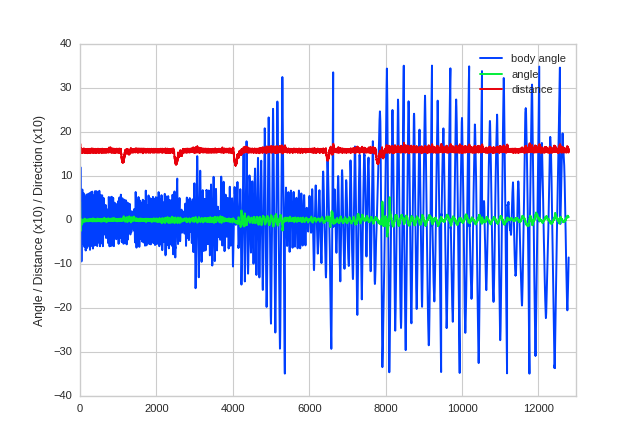
\includegraphics[scale=0.77]{figures/plots/newPlots/base2_perf}%perfdvsOnlyB2}
  \caption{ Single Layer Network + Head Control: performance in training }
  \label{fig:perfdvsOnlyB2}
\end{figure}
\begin{figure}[htpb]
  \centering
  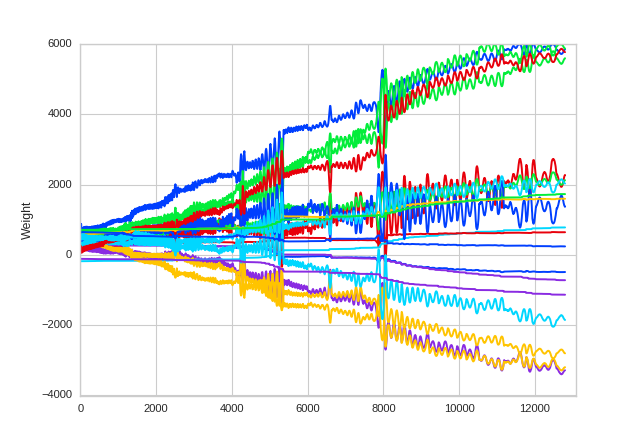
\includegraphics[scale=0.77]{figures/plots/newPlots/base2_weights}%wblWbrB2Dvs}
  \caption{ Single Layer Network + Head Control: Plot of the weights }
  \label{fig:wblWbrB2Dvs}
\end{figure}
\subsection{Additional Tests}
Having this result additional setups of single layer SNNs with different inputs for the neurons controlling the direction where tested. In the first setup these were connected additionally to the output neurons for head control. In the second setup the input of the body neurons consisted of two neurons each for the first, third and fifth joint of the snake, decoding its angle as described in \autoref{sec:EnOfJoint} and as before the connections to the head output neurons. The other parameters were kept the same.
Both networks showed a similar behavior to the first test case with head control and seem not to be able to solve the task using additional and different inputs. \autoref{fig:baADistB2DvsH} and \autoref{fig:baADistB2JointH} show the mean angles for these two runs and how their performance gets worse over time.

\begin{figure}[htpb]
  \centering
  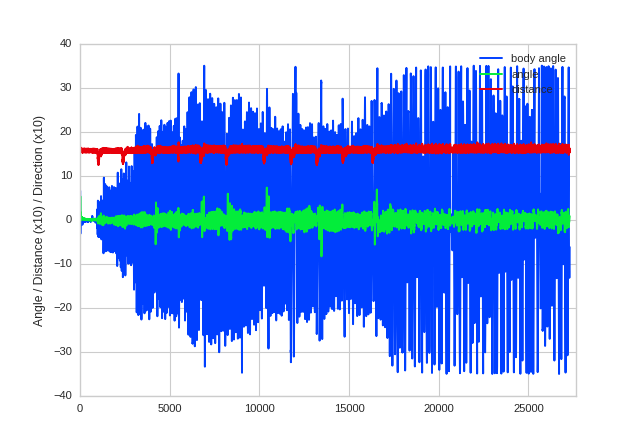
\includegraphics[scale=0.77]{figures/plots/newPlots/base2HJoints_perf}%baADistB2JointH}
  \caption{ Performance of SNN with Joint Angles and Head output as input (training) }
  \label{fig:baADistB2JointH}
\end{figure}
\begin{figure}[htpb]
  \centering
  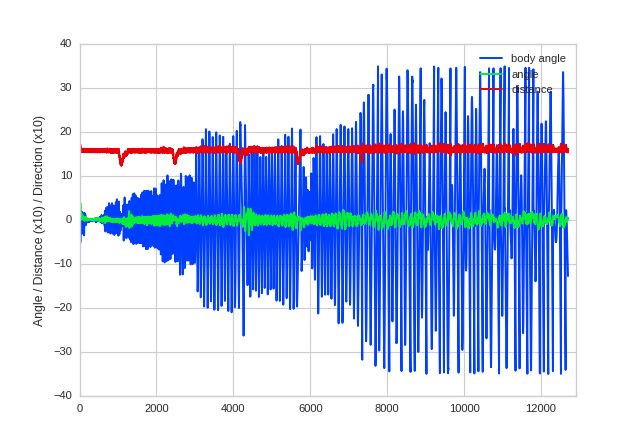
\includegraphics[scale=0.77]{figures/plots/newPlots/base2HDVS_perf}%baADistB2DvsH}
  \caption{ Performance of SNN with DVS and Head output as input (training)  }
  \label{fig:baADistB2DvsH}
\end{figure}

\section{Multi layer Networks}
Previous experiments suggest that a single layered network lacks complexity to solve this task and thus the next experiments will use a second, hidden layer. As the control of the head worked good in the last three examples the head output neurons get still directly connected to only the dvs layer and rewarded as before. Similar to the last experiment six neurons encoding the joint angles and the two output neurons of the head control are used for the input of the hidden layer. The idea behind this is that the output of the head neurons should in some degree encode the information from the DVS input and the angles of the joints but especially the angle of the head joint describe the state of the body. The first, third and fifth joint are chosen as these are the first joints responsible for horizontal movement in the slithering gate of the snake.

\subsection{Single Hidden Layer}
In the first multilayered setup the hidden layer consists of eight neurons, which is the same amount as it has inputs, and the two layers are connected in an ‘all-to-all’ fashion. The parameters for the hidden neurons are shown in \autoref{tab:M1hiddenN} with the main difference in their capacity being higher than previews neurons. For synapses between the input and the hidden layer the parameters shown in \autoref{tab:M1SynH} are used. $tau_{c}$ is set to a higher value compared to previews synapses, with the effect that the eligibility is accumulated over a larger time span and thus the synapse remembers its responsibility for triggering the neuron it connects to for a longer time. This would result in a higher absolute value for the eligibility which would lead to drastic changes of the weights; to counteract this the values for the positive and the negative STDP learning window are scaled down by the same factor $tau_{c}$ is scaled up. For the assignment of the reward to each hidden neuron the backpropagation method described in \autoref{sec:rewardAss} is used and the reward is calculated by \autoref{eq:rewardPSimp}. The parameters used for the connections from the hidden layer to the output for the body are shown in \autoref{tab:M1SynOb}, the topologie of the network is displayed in \autoref{fig:M1netTop}.

\begin{figure}[htpb]
  \centering
  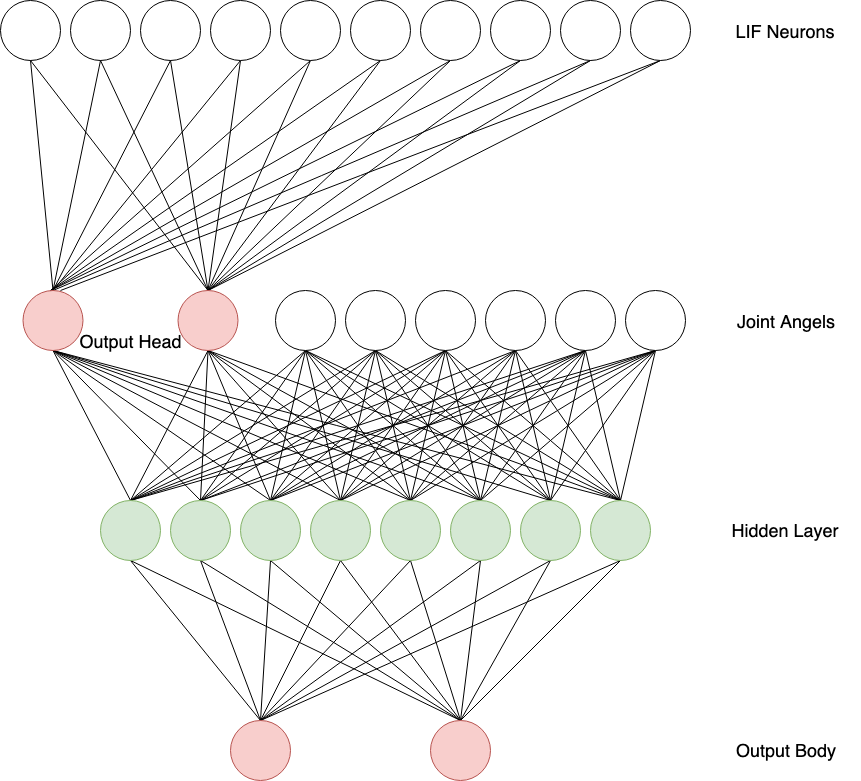
\includegraphics[width=\textwidth]{figures/plots/M1NetworkTop}
  \caption{ Sketch of Network Topology for the Network with one hidden layer  }
  \label{fig:M1netTop}
\end{figure}

% \def\layersep{2.5cm}
% \begin{tikzpicture}[shorten >=1pt,->,draw=black!50, node distance=\layersep]
%   \tikzstyle{every pin edge}=[<-,shorten <=1pt]
%   \tikzstyle{neuron}=[circle,fill=black!25,minimum size=17pt,inner sep=0pt]
%   \tikzstyle{input neuron}=[neuron, fill=green!50];
%   \tikzstyle{output neuron}=[neuron, fill=red!50];
%   \tikzstyle{hidden neuron}=[neuron, fill=blue!50];
%   \tikzstyle{annot} = [text width=4em, text centered]

%   % Draw the input layer nodes
%   \foreach \name / \y in {1,...,16}
%   % This is the same as writing \foreach \name / \y in {1/1,2/2,3/3,4/4}
%       \node[input neuron, pin=left:Input \#\y] (I-\name) at (0,-\y) {};

%   % Draw the hidden layer nodes
%   \foreach \name / \y in {1,...,8}
%       \path[yshift=0.5cm]
%           node[hidden neuron] (H-\name) at (\layersep,-\y cm) {};

%   % Draw the output layer node
%   \foreach \name / \y in {1,...,4}
%     \node[output neuron,pin={[pin edge={->}]right:Output \#\y}, right of=H-3] (\layersep*2,-\y) {};

%   % Connect every node in the input layer with every node in the
%   % hidden layer.
%   \foreach \source in {1,...,10}
%       \foreach \dest in {1,...,2}
%           \path (I-\source) edge (O-\dest);

%   % Connect every node in the hidden layer with the output layer
%   \foreach \source in {1,...,5}
%       \path (H-\source) edge (O);

%   % Annotate the layers
%   \node[annot,above of=H-1, node distance=1cm] (hl) {Hidden layer};
%   \node[annot,left of=hl] {Input layer};
%   \node[annot,right of=hl] {Output layer};
% \end{tikzpicture}


\begin{table}[htpb]
  \centering
  \caption[Parameters Single Hidden Layer]{Parameters of the hidden synapses for the single hidden layer setup} \label{tab:M1SynH}
  \begin{tabular}{|c| c |l|}
      \toprule
      Parameter  & Value & Description \\
      \midrule
      $W_{max}$ & 6000   & Maximum weight of synapse\\   
      $W_{min}$ & -6000  & Minimum weight of synapse\\   
      $A_{+}$   & 0.002    & Constant scaling strength of potentiation\\   
      $A_{-}$   & -0.001   & Constant scaling strength of depression \\   
      $\tau_c$  & 10000.0   & Time constant of eligibility trace \\  
      $\tau_n$  & 20.0   & Time constant of reward signal  \\   
      $b$       & 0.0    & Baseline neuromodulator concentration \\    
      \bottomrule
  \end{tabular}
\end{table}
  
  \begin{table}[htpb]
  \centering
  \caption[Parameters 2.Setup]{Parameters of hidden Neurons for the single hidden layer setup} \label{tab:M1hiddenN}
    \begin{tabular}{|c| c |l|}
      \toprule
      Parameter & Value & Description \\
      \midrule
      $c_m$   & 100.0  & Capacity of the membrane \\
      $tau_{m}$    & 50.0  & Membrane time constant \\
      $tau_{refrac}$   & 1.  & Duration of refractory period\\
      $v_{thresh}$   & -50.0  & Spike initiation threshold \\
      $v_{reset}$    & -65.0  &  Reset value for $V_m$ after a spike \\
      $v_{rest}$ & -65.0 & Resting voltage for $V_m$ \\
      \bottomrule
    \end{tabular}
  \end{table}

  \begin{table}[htpb]
  \centering
  \caption[Parameters Single Hidden Layer]{Parameters of the body output synapses for the single hidden layer setup} \label{tab:M1SynOb}
    \begin{tabular}{|c| c |l|}
        \toprule
        Parameter  & Value & Description \\
        \midrule
        $W_{max}$ & 6000   & Maximum weight of synapse\\   
        $W_{min}$ & -6000  & Minimum weight of synapse\\   
        $A_{+}$   & 0.2    & Constant scaling strength of potentiation\\   
        $A_{-}$   & -0.1   & Constant scaling strength of depression \\   
        $\tau_c$  & 100.0   & Time constant of eligibility trace \\  
        $\tau_n$  & 20.0   & Time constant of reward signal  \\   
        $b$       & 0.0    & Baseline neuromodulator concentration \\    
        \bottomrule
    \end{tabular}
  \end{table}
For this setup the learning phase was much longer compared to the single layer network. At the time the weights for the first setup stabilised the weights in this simulation still were under a lot of change. This can be seen by comparing the graph of the weights for the output layer in \autoref{fig:WBase1}, with \autoref{fig:M1Wb} which shows the weights for this setup.
\begin{figure}[htpb]
  \centering
  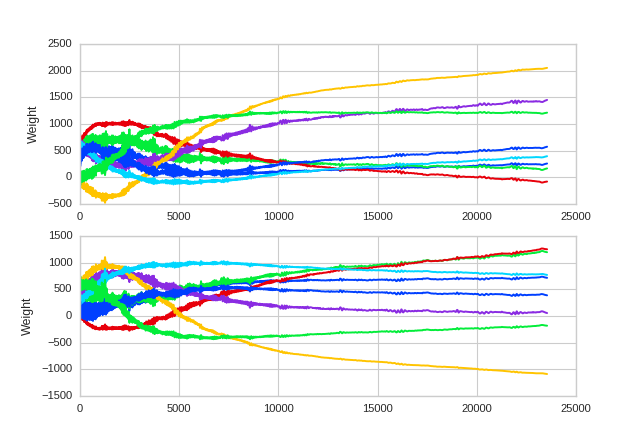
\includegraphics[width=\textwidth]{figures/plots/newPlots/m1Train_bodyW}%M1Wb}
  \caption{ Weights connecting the body output of SNN with the hidden Layer (training)  }
  \label{fig:M1Wb}
\end{figure}
While the changes get less over time the network remains able to solve the task with a very good performance of the head and a good result for the mean body angle with peaks of around $25$ degrees towards the end of the training. \autoref{fig:M1baADist} shows the plot of the mean angles as well as the distance to the target for this setup.
\begin{figure}[htpb]
  \centering
  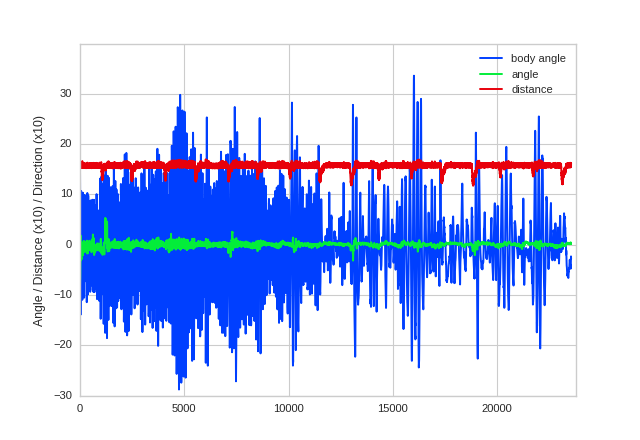
\includegraphics[width=\textwidth]{figures/plots/newPlots/m1train_perf}%M1baADist}
  \caption{ Performance of SNN with one hidden Layer (training)  }
  \label{fig:M1baADist}
\end{figure}
\subsection{Split Hidden Layer}
The last network trained is similar to the previous network in all parameters, the only difference lies in the topologie of the network. As shown in \autoref{fig:M2netTop} the hidden layer is split in two pairs of four neurons each and all outgoing connections from a pair go to only one neuron in the output layer. \autoref{eq:rewardPSimp} simplifies for this setup to

\begin{figure}[htpb]
  \centering
  \includegraphics[width=\textwidth]{figures/plots/M2netTop}
  \caption{ Sketch of Network Topology for the Network with split hidden layer  }
  \label{fig:M2netTop}
\end{figure}

\begin{equation}
r_h = r * \frac{w_r} {|w_r|)}
\end{equation}
for the hidden layer connected to the right output and
\begin{equation}
r_h = - r * \frac{w_l} {|w_l|)}
\end{equation}
for the hidden layer connected to the left output. This simplification is the result of hidden neurons influencing only one other neuron. In this equitations $w_l$/$w_r$ are the weights of the connection from a neuron in left/right hidden layer to its output and $r$ is the reward for the output, calculated as before.
Training the network took about as long as for the other multilayered network and the overall performance is comparable but this version had spikes in the mean body angle of around $32$ degrees. The plot of the mean angles for this training is shown in \autoref{fig:baADistMS}.
\begin{figure}[htpb]
  \centering
  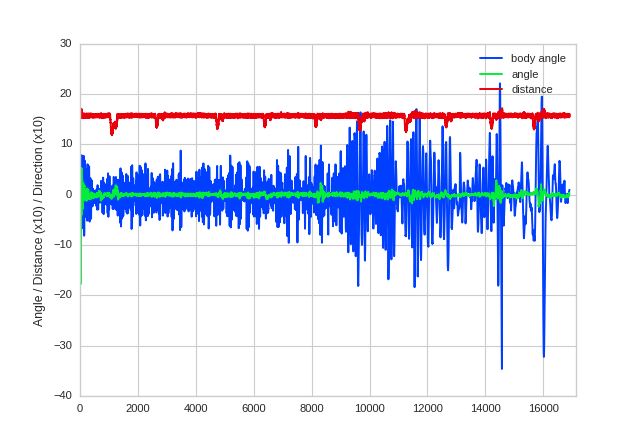
\includegraphics[width=\textwidth]{figures/plots/newPlots/m2-train_perf}%baADistMS}
  \caption{ Performance of SNN with a split hidden Layer (training)  }
  \label{fig:baADistMS}
\end{figure}
